\documentclass[10pt]{article}
\usepackage[letterpaper,text={6.5in,8.7in},centering]{geometry}
\usepackage{epic,eepic}
\usepackage{amssymb,amsmath,times,subfigure,graphicx,theorem}
%\usepackage{warmread}
%\usepackage[all,import]{xy}
%\usepackage{eepic}
\usepackage{subfigure}

\usepackage{amsmath}
\newcommand{\argmax}{\operatornamewithlimits{argmax}}

\newcommand{\norm}[1]{\ensuremath{\left\| #1 \right\|}}
\newcommand{\bracket}[1]{\ensuremath{\left[ #1 \right]}}
\newcommand{\braces}[1]{\ensuremath{\left\{ #1 \right\}}}
\newcommand{\parenth}[1]{\ensuremath{\left( #1 \right)}}
\newcommand{\pair}[1]{\ensuremath{\langle #1 \rangle}}
\newcommand{\met}[1]{\ensuremath{\langle\langle #1 \rangle\rangle}}
\newcommand{\refeqn}[1]{(\ref{eqn:#1})}
\newcommand{\reffig}[1]{Figure \ref{fig:#1}}
\newcommand{\tr}[1]{\mathrm{tr}\ensuremath{\negthickspace\bracket{#1}}}
\newcommand{\trs}[1]{\mathrm{tr}\ensuremath{[#1]}}
\newcommand{\deriv}[2]{\ensuremath{\frac{\partial #1}{\partial #2}}}
\newcommand{\SO}{\ensuremath{\mathsf{SO(3)}}}
\newcommand{\T}{\ensuremath{\mathsf{T}}}
\renewcommand{\L}{\ensuremath{\mathsf{L}}}
\newcommand{\so}{\ensuremath{\mathfrak{so}(3)}}
\newcommand{\SE}{\ensuremath{\mathsf{SE(3)}}}
\newcommand{\se}{\ensuremath{\mathfrak{se}(3)}}
\renewcommand{\Re}{\ensuremath{\mathbb{R}}}
\newcommand{\aSE}[2]{\ensuremath{\begin{bmatrix}#1&#2\\0&1\end{bmatrix}}}
\newcommand{\ase}[2]{\ensuremath{\begin{bmatrix}#1&#2\\0&0\end{bmatrix}}}
\newcommand{\D}{\ensuremath{\mathbf{D}}}
\newcommand{\Sph}{\ensuremath{\mathsf{S}}}
\renewcommand{\S}{\Sph}
\newcommand{\J}{\ensuremath{\mathbf{J}}}
\newcommand{\Ad}{\ensuremath{\mathrm{Ad}}}
\newcommand{\intp}{\ensuremath{\mathbf{i}}}
\newcommand{\extd}{\ensuremath{\mathbf{d}}}
\newcommand{\hor}{\ensuremath{\mathrm{hor}}}
\newcommand{\ver}{\ensuremath{\mathrm{ver}}}
\newcommand{\dyn}{\ensuremath{\mathrm{dyn}}}
\newcommand{\geo}{\ensuremath{\mathrm{geo}}}
\newcommand{\Q}{\ensuremath{\mathsf{Q}}}
\newcommand{\G}{\ensuremath{\mathsf{G}}}
\newcommand{\g}{\ensuremath{\mathfrak{g}}}
\newcommand{\Hess}{\ensuremath{\mathrm{Hess}}}

\renewcommand{\baselinestretch}{1.2}
\date{}

\renewcommand{\thesubsection}{\arabic{subsection}. }
\renewcommand{\thesubsubsection}{\arabic{subsection}.\arabic{subsubsection} }

\theoremstyle{plain}\theorembodyfont{\normalfont}
\newtheorem{prob}{Question}[section]
%\renewcommand{\theprob}{\arabic{section}.\arabic{prob}}
\renewcommand{\theprob}{\arabic{prob}}

\newenvironment{subprob}%
{\renewcommand{\theenumi}{\alph{enumi}}\renewcommand{\labelenumi}{(\theenumi)}\begin{enumerate}}%
{\end{enumerate}}%


\begin{document}

\section{Optimal Joint Probabilistic Data Assocation Filter (O-JPDAF)}

%\section*{Coalescence Avoiding Optimal Joint Probabilistic Data Association Filter (C-JPDAF)}
%
%The difference between the JPDAF and the C-JPDAF is that the JPDAF is optimal in the sence that estimate uncertainty is minimized. However, the C-JPDAF minimizes a weighted sum of uncertainty and similarity to decrease track coalescence, from which the JPDAF suffers when estimates are in close proximity over long periods of time.

% Paper copy & paste starts below:

\subsection{Flow Update}
Similar to Kalman filters, the JPDAF is composed of a flow update and a measurement update. During the flow update (or prediction step), the estimated state $\hat x_{i_k}$ and its covariance $P_{i_k}$ for each track $i=\{1,2,...,t\}$ of $t$ tracks at time step $k$ is updated as follows:
\begin{gather}
\hat x_{i_{k}} = f_{i_{k-1}}( \hat x_{i_{k-1}}),\\
P_{i_{k}} = F_{i_{k-1}} P_{i_{k-1}} F_{i_{k-1}}^T + Q_{i_{k-1}}, \quad F_{i_{k-1}}=\frac{\partial f}{\partial x}\bigg|_{x=\hat x_{i_{k}} }
\end{gather}
where the uncertainty of the process is represented with covariance $Q_{i_{k-1}}$.
These equations are applied between measurements to provide predictions of the states and their uncertainties. % paper change

\subsection{Measurement Update}

The measurement serves to update the state estimate. Because all equations in this section take place at the $k$ time step, this subscript is removed from the equations. Let  the a priori value of a variable and its a posteriori value be denoted by the superscript $-$ and $+$, respectively. Let subscript $j$ indicate a measurement index such that the set $j=\{1,2,...,r\}$ for the number of returns $r$ (or measurements). For a given measurement $z_j$, its measurement residual or innovation for the $i$-th object is given by
\begin{align*}
e_{ij} = z_j - \hat z_i
\end{align*}
where $\hat z_i$ is the predicted measurement of the linearized equation
\begin{align}
\hat z_i = H_i \hat x_{i}^-
\end{align}
such that the measurement is a function of state
\begin{align}
z=h(x), \quad H_i=\frac{\partial h}{\partial x}\bigg|_{x=\hat x_{i_{k}}^- }.
\end{align}•
Given the uncertainty of the measurements represented with covariance $R_i$, the innovation covariance $S_{i}$ is
\begin{align}
S_{i}=H_{i}P_{i}^{-}H_{i}^T+R_{i}.
\end{align}


% [Eq. 1.4.16-(1-10)]


\subsubsection{Likelihood of Association}
The computation required with a standard JPDA is inconsistent with the capabilities of the computational resources to account for an arbitrary number of objects to be tracked~\cite[Eq. 1.(1-2)]{Bar1990}. A modified version of the JPDA, commonly known as the "Cheap JPDA", provides a simpler approximation of the likelihood $\beta_{ij}$ that a return $j$ (or measurement) belongs to a particular track $i$ (or object). We define $G_{ij}$, which takes a very similar form as the Gaussian probability density function
\begin{align}
G_{ij}=\frac1{\sqrt{\det{S_{ij}}}}\exp{\{-\frac12e_{ij}^TS_{ij}^{-1}e_{ij}\}}
\end{align}
which is used to calculate the probability of association $\beta_{ij}$ as well as intermediate variables $\mathcal{S}_{ti}$ and $\mathcal{S}_{ri}$
\begin{align}
\beta_{ij}=\frac{G_{ij}}{\mathcal{S}_{ti}+\mathcal{S}_{ri}-G_{ij}+B}, 
\quad 
\mathcal{S}_{ti}=\sum\limits_{j}G_{ij}, 
\quad 
\mathcal{S}_{ri}=\sum\limits_{i}G_{ij}
\end{align}
where $B$ is a correction factor to account for the nonunity probability of detection as well as clutter and false alarms. Unless there are reasons that either phenomena may occur, we assume $B=0$.

\subsubsection{State and Covariance Update Equations}
The weighted sum of all innovations associated with the object $i$ is defined as ${\bf{e}}_{i}={\sum\limits_{j} \beta_{ij}e_{ij}}$.
The resulting a posteriori estimate of the state is given by~\cite[Eq. 6-(25-26)]{TrackDataAssoc}
\begin{align}
\hat x^+_{i}=&\hat x^-_{i}+K_{i}{\bf{e}}_{i}\label{eqn:KalEst}
\end{align}
where $K_i$ is a gain chosen to minimize the a posteriori uncertainty of the state estimate; $K_i$ is derived below optimally in the sence that the a posteriori uncertainties are minimized with respect to the generalized linearized equations of a JPDAF. Of course, the estimator cannot be optimal if the system is nonlinear, because the linearized equations to not fully represent the dynamics of a nonlinear system.

We define the likelihood that object $i$ is not detected is $\beta_{0,i}=1-{\sum\limits_{j} \beta_{ij}}$. The resulting a posteriori covariance can be written as [Tracking and Data Association, pg. 326, equations D-32 and D-33]
\begin{align}
\label{eqn:JPDAFCov}
P^+_{i}=& \beta_{0,i}P^-_{i}+(1-\beta_{0,i})P_i^c+\tilde P
\\
\tilde P=&K_i\left({\sum\limits_{j} \beta_{ij}e_{ij}e_{ij}^T-{\bf{e}}_{i}}{\bf{e}}_{i}^T\right)K_{i}^T\label{eqn:tildeP}
\end{align}
where $P_i^c$ is defined as the a posteriori covariance of object $i$ if only a single measurement serves to update this track.
%From [Tracking and Data Association, pg. 326, equation D-27], which is referenced in numerous publications, $P_i^c$ is calculated
%\begin{align}
%\label{eqn:PcKalman1}
%P_i^c=(I-K_{i,Kalman}H_i)P_i^-
%\end{align}
%or equivalently
%\begin{align}
%\label{eqn:PcKalman2}
%P_i^c=P_i^--K_{i,Kalman}SK_{i,Kalman}^T
%\end{align}
%where Kalman gain $K_{i,Kalman}=P_iH_i^TS_i^{-1}$ is used. In fact, (\ref{eqn:PcKalman1}) and (\ref{eqn:PcKalman2}) are derived from equations that require $K_{i,Kalman}$ be used. Below we show that $K_{i,Kalman}$ cannot guarantee that $\tr{P^+_{i}}$ is minimized:
%\begin{align}
%P^+_{i}=& \beta_{0,i}P^-_{i}+(1-\beta_{0,i})\left(P_i^--K_{i,Kalman}SK_{i,Kalman}^T\right)+K_{i,Kalman}\left({\sum\limits_{j} \beta_{ij}e_{ij}e_{ij}^T-{\bf{e}}_{i}}{\bf{e}}_{i}^T\right)K_{i,Kalman}^T\\
%=&P^-_{i}-K_{i,Kalman}\left((1-\beta_{0,i})S-({\sum\limits_{j} \beta_{ij}e_{ij}e_{ij}^T-{\bf{e}}_{i}}{\bf{e}}_{i}^T)\right)K_{i,Kalman}^T\\
%=&P^-_{i}-K_{i,Kalman}S^*K_{i,Kalman}^T, \quad S^*=(1-\beta_{0,i})S-({\sum\limits_{j} \beta_{ij}e_{ij}e_{ij}^T-{\bf{e}}_{i}}{\bf{e}}_{i}^T).
%\end{align}
%We define the cost function $J^*=\tr{K_{i,Kalman}}$ to test for optimality with respect to $K_i$ assuming that $K_i=K_{i,Kalman}$ to show if this is true:
%\begin{align}
%0&=\frac{\partial\tr{P^+_i}}{\partial K_i}
%\\
%0&=-2(1-\beta_{0,i})\frac{\partial\tr{K_iH_iP^-_i}}{\partial K_i}+\frac{\partial\tr{K_iS^*K_i^T}}{\partial K_i}
%\\
%0&=-2(1-\beta_{0,i})P^-_iH_i^T+2K_iE_i
%\\
%K_iE_i&=(1-\beta_{0,i})P^-_iH_i^T
%\\
%K_i&=(1-\beta_{0,i})P^-_iH_i^TE_i^{-1}\label{eqn:GainK}
%\end{align}
We can define $P_i^c$ without any assumptions on $K_i$ (i.e. $K_i$ is not necessarily the Kalman gain, so the well-known Kalman covariance update equations are not valid here) [Applied Optimal Estimation, pg. 108, equation 4.2-12]
\begin{align}
\begin{split}
P^c_i&=(I-K_iH_i)P^-_i(I-K_iH_i)^T+K_iR_iK_i^T
\\
&=P^-_i-(K_iH_iP^-_i+P^-_iH_i^TK_i^T)+K_i(H_iP^-_iH_i^T+R_i)K_i^T.
\label{eqn:GenCov}
\end{split}
\end{align}
Substituting \refeqn{tildeP} and \refeqn{GenCov} into \refeqn{JPDAFCov},
\begin{align}
\begin{split}
P^+_{i}=&\beta_{0,i}P^-_{i}+(1-\beta_{0,i})\left(P^-_i-(K_iH_iP^-_i+P^-_iH_i^TK_i^T)+K_i(H_iP^-_iH_i^T+R_i)K_i^T\right)\\&+K_i\left({\sum\limits_{j} \beta_{ij}e_{ij}e_{ij}^T-{\bf{e}}_{i}}{\bf{e}}_{i}^T\right)K_{i}^T
\end{split}
\\
\begin{split}
P^+_{i}=&P^-_{i}-(1-\beta_{0,i})(K_iH_iP^-_i+P^-_iH_i^TK_i^T)\\&+K_i\left((1-\beta_{0,i})(H_iP^-_iH_i^T+R_i)+{\sum\limits_{j} \beta_{ij}e_{ij}e_{ij}^T-{\bf{e}}_{i}}{\bf{e}}_{i}^T\right)K_i^T
\end{split}
\\
\begin{split}
P^+_{i}=&P^-_{i}-(1-\beta_{0,i})(K_iH_iP^-_i+P^-_iH_i^TK_i^T)+K_iE_iK_i^T,\\
&E_i=(1-\beta_{0,i})(H_iP^-_iH_i^T+R_i)+{\sum\limits_{j} \beta_{ij}e_{ij}e_{ij}^T-{\bf{e}}_{i}}{\bf{e}}_{i}^T\label{eqn:CovExpanded}
\end{split}
\end{align}
where $E_i=E_i^T$ and may be calculated without knowledge of the gain matrix $K_i$, and is invertible because $P^-_i$ and $R_i$ are positive-definite and $(\beta_{ij}e_{ij}e_{ij}^T-{\bf{e}}_{i}{\bf{e}}_{i}^T)$ are positive-semidefinite, shown below. 

Consider that object $i$ is not measured (likelihood $\beta_{0,i}$), then this portion of the innovation update $e_0=0_{m\times1}$ because no innovation exists where measurments are not available. Then for all innovations in the set $j^*=\{0,1, 2,...,r\}$, the Total Probability Theorem holds true for object $i$:
\begin{align}
\sum\limits_{j^*}\beta_{ij^*}=1.
\end{align}
From~\cite[Eq. 1.4.16-(1-10)]{ShaRonThi2001}, the covariance spread in the means term of the mixture of $e$ is defined as (note that ${\bf e}_{i}$ remains unchanged)
\begin{align}
\tilde P_e=\sum\limits_{j^*}\beta_{ij^*}(e_{ij^*}-{\bf e}_{i})(e_{ij^*}-{\bf e}_{i})^T
\end{align}
which is positive semi-definite. Manipulating this equation,
\begin{align}
\tilde P_e&=\sum\limits_{j^*}\beta_{ij^*}e_{ij^*}e_{ij^*}^T
-\sum\limits_{j^*}\beta_{ij^*}e_{ij^*}{\bf e}_{i}^T
-{\bf e}_{i}\sum\limits_{j^*}\beta_{ij^*}e_{ij^*}^T
+{\bf e}_{i}{\bf e}_{i}^T
\\
\tilde P_e&=\sum\limits_{j^*}\beta_{ij^*}e_{ij^*}e_{ij^*}^T-{\bf e}_{i}{\bf e}_{i}^T
\\
\tilde P_e&=\sum\limits_{j}\beta_{ij}e_{ij}e_{ij}^T-{\bf e}_{i}{\bf e}_{i}^T\geq0
\label{eqn:CovSpreadPSD}
\end{align}
because $e_{ij^*}\equiv0$. Therefore $E_i$ is invertible $\forall\ \beta_{0,i}<1$.



The only other case where $E_i$ is not invertible is when $\beta_{0,i}=1$, or when there is full confidence that a particular object is not observed by any measurement. This case is evaluated after the gain matrix is derived.

The goal of the choosing $K_i$ is to minimize the uncertainty of the object state. With a Kalman filter, this goal is accomplished by minimizing $\tr{P^+_i}$ with respect to $K_i$ such that the total number of tracks $t=1$; the same approach may be applied to the JPDAF, except the a posteriori covariance equation has changed, so $K_i$ changes as well ($t=1$ is not guaranteed):
\begin{align}
0&=\frac{\partial\tr{P^+_i}}{\partial K_i}
\\
0&=-2(1-\beta_{0,i})\frac{\partial\tr{K_iH_iP^-_i}}{\partial K_i}+\frac{\partial\tr{K_iE_iK_i^T}}{\partial K_i}
\\
0&=-2(1-\beta_{0,i})P^-_iH_i^T+2K_iE_i\label{eqn:Uncertainty0}
\\
K_iE_i&=(1-\beta_{0,i})P^-_iH_i^T
\\
K_i&=(1-\beta_{0,i})P^-_iH_i^TE_i^{-1}\label{eqn:GainK}
\end{align}
such that \refeqn{GainK} may be substituted into \refeqn{CovExpanded}
\begin{align}
\begin{split}
P^+_{i}=&P^-_{i}-(1-\beta_{0,i})^2(P^-_iH_i^TE_i^{-1}H_iP^-_i+P^-_iH_i^TE_i^{-1}H_iP^-_i)
\\
&+(1-\beta_{0,i})^2P^-_iH_i^TE_i^{-1}E_iE_i^{-1}H_iP^-_i
\end{split}
\\
P^+_{i}=&P^-_{i}-(1-\beta_{0,i})^2P^-_iH_i^TE_i^{-1}H_iP^-_i
\end{align}
which may be simplified in two ways
\begin{align}
P^+_{i}=&P^-_{i}-K_iE_iK_i^T,\label{eqn:JPDAFPostCovSymmetricUpdate}
\\
P^+_{i}=&\left(I-(1-\beta_{0,i})K_iH_i\right)P^-_i.\label{eqn:JPDAFPostCovSimpleUpdate}
\end{align}

Consider the singularity when $E_i=0$ if no association is made to a track, or where $(1-\beta_{0,i})=\sum\limits_{j}\beta_j=0$.
While it is clear from \refeqn{KalEst} and \refeqn{CovExpanded} that the updates are independent of $K_i$ at this singularity, we show that $K_i$ is not growing without bound nearby the singularity.
Hence, we evaluate the limit at this singularity to ensure it is not infinite.
Note that if $\sum\limits_{j}\beta_j\rightarrow0\Rightarrow \beta_j\rightarrow0\ \forall j$ because of the bounds $\sum\limits_{j}\beta_j\geq\beta_j\geq0\ \forall j$. For clarity, let $\beta^*=\sum\limits_{j}\beta_j$ and let $\tilde\beta_p=\sum\limits_{j,j\neq p}\beta_j/\sum\limits_{j}\beta_j$ and we drop the subscript $i$ because this analysis focuses on a single track. First we evaluate the summations inside $E$, then consider the effect on $K$:
\begin{align}
\begin{split}
&\sum\limits_{j} \beta_{j}e_{j}e_{j}^T=(\beta_1e_1e_1^T+\beta_2e_2e_2^T+...)
\\
&=(\beta_1+\beta_2+...)
(e_1e_1^T-\tilde\beta_1e_1e_1^T+
e_2e_2^T-\tilde\beta_2e_2e_2^T+...)
\\
&=\beta^*(\sum\limits_{j}e_{j}e_{j}^T-\sum\limits_{j}\tilde\beta_je_{j}e_{j}^T)
\end{split}
\\
\begin{split}
&{{\bf{e}}}{\bf{e}}^T=\sum\limits_{j} \beta_{j}e_{j}\sum\limits_{j} \beta_{j}e_{j}^T=
(\beta_1e_1\sum\limits_{j} \beta_{j}e_{j}^T+\beta_2e_2\sum\limits_{j} \beta_{j}e_{j}^T+...)
\\
&=(\beta_1+\beta_2+...)(e_1\sum\limits_{j} \beta_{j}e_{j}^T-\tilde\beta_1e_1\sum\limits_{j} \beta_{j}e_{j}^T+
e_2\sum\limits_{j} \beta_{j}e_{j}^T-\tilde\beta_2e_2\sum\limits_{j} \beta_{j}e_{j}^T+...)
\\
&=\beta^*(\sum\limits_{j}e_{j}\sum\limits_{j}\beta_je_{j}^T-\sum\limits_{j}\tilde\beta_je_{j}\sum\limits_{j}\beta_je_{j}^T)
\end{split}
\\
\begin{split}
&\lim_{\beta^* \to 0}K=\lim_{\beta^* \to 0}\beta^*P^-H^T
\left(\beta^*[S+\sum\limits_{j}e_{j}e_{j}^T-\sum\limits_{j}\tilde\beta_je_{j}e_{j}^T-\sum\limits_{j}e_{j}\sum\limits_{j}\beta_je_{j}^T+\sum\limits_{j}\tilde\beta_je_{j}\sum\limits_{j}\beta_je_{j}^T]\right)^{-1}
\\
&=P^-H^T\lim_{\beta^* \to 0}
\left(S+\sum\limits_{j}e_{j}e_{j}^T-\sum\limits_{j}\tilde\beta_je_{j}e_{j}^T-\sum\limits_{j}e_{j}\sum\limits_{j}\beta_je_{j}^T+\sum\limits_{j}\tilde\beta_je_{j}\sum\limits_{j}\beta_je_{j}^T\right)^{-1}
\label{eqn:OptGainNoSingularity}
\end{split}
\end{align}
which not an infinite limit because of the following bounded conditions:
\begin{align}
\begin{split}
&\lim_{\beta^* \to 0}\tilde\beta_p=\lim_{\beta^* \to 0}\frac{\beta_1+\beta_2+...+\beta_{p-1}+0+\beta_{p+1}+...}{\beta_1+\beta_2+...+\beta_{p-1}+\beta_p+\beta_{p+1}+...}\ \forall p\in j
\\
&=1-\lim_{\beta^* \to 0}\frac{\beta_p}{\beta^*},\quad 0\leq\beta_p\leq\beta^*\leq1\Rightarrow0\leq\lim_{\beta^* \to 0}\frac{\beta_p}{\beta^*}\leq1\Rightarrow0\leq\lim_{\beta^* \to 0}\tilde\beta_p\leq1.
\end{split}
\end{align}
and therefore \refeqn{OptGainNoSingularity} may be solved
\begin{align}
\lim_{\beta^* \to 0}K&=P^-H^T
\left(S+\sum\limits_{j}e_{j}e_{j}^T-\sum\limits_{j}{B_j}e_{j}e_{j}^T\right)^{-1}
\\
&=P^-H^T
\left(S+\sum\limits_{j}(1-B_j)e_{j}e_{j}^T\right)^{-1}
\label{eqn:OptGainNoSingularitySolved}
\end{align}
for $0\leq B_j\leq1\ \forall j$ and it can be easily seen that the sum of the terms inside the parentheses are invertible.
% and we know that $S+\sum\limits_{j}e_{j}e_{j}^T-\sum\limits_{j}{B_j}e_{j}e_{j}^T$ is invertible because $S$ is positive definite and the remaining terms are a simplified form of \refeqn{CovSpreadPSD}.
From a computational standpoint, for every $\beta^*_i\approx0$, the effect of the measurement update should be negligible, so we may choose $K_i=0_{n\times m}$ near this singularity as it will have little effect on the filter performance. Choosing $K_i$ this way results in no difference between the a priori and a posteriori update results (no measurement update where no measurement is observed). 
%\begin{align}
%\begin{split}
%\lim_{\beta^* \to 0}K&=\lim_{\beta^* \to 0}P^-H^T
%\left(S+\sum\limits_{j}e_{j}e_{j}^T-\sum\limits_{j}\tilde\beta_je_{j}e_{j}^T-\sum\limits_{j}e_{j}\sum\limits_{j}\beta_je_{j}^T+\sum\limits_{j}\tilde\beta_je_{j}\sum\limits_{j}\beta_je_{j}^T\right)^{-1}
%\\
%&asfd
%\end{split}
%\end{align}

We show that the Kalman gain $K_{Kalman}$ and the optimal JPDAF gain $K_{O-JPDAF}$ are not always the same with a proof by contradiction. Consider that these gains are equivalent (object subscript $i$ is omitted for clarity):
\begin{align}
&K_{Kalman}=K_{O-JPDAF}
\\
&P^-H^TS^{-1}=(1-\beta_{0})P^-H^TE^{-1}
\\
&P^-H^TS^{-1}E=(1-\beta_{0})P^-H^T
\\
&P^-H^TS^{-1}\left((1-\beta_{0})S+{\sum\limits_{j} \beta_{j}e_{j}e_{j}^T-{\bf{e}}}{\bf{e}}^T\right)=(1-\beta_{0})P^-H^T
\\
&(1-\beta_{0})P^-H^T+P^-H^TS^{-1}\left({\sum\limits_{j} \beta_{j}e_{j}e_{j}^T-{\bf{e}}}{\bf{e}}^T\right)=(1-\beta_{0})P^-H^T
\\
&K_{Kalman}\left({\sum\limits_{j} \beta_{j}e_{j}e_{j}^T-{\bf{e}}}{\bf{e}}^T\right)=0.\label{eqn:ContradictionResult}
\end{align}

The final statement implies that the spread in the innovations $\tilde P\equiv0$, which is not assumed in the JPDAF. The result of \refeqn{ContradictionResult} may only occur if $K_{Kalman}=0$, the probabilities that each measurement $j$ belongs to each object $i$ is exactly $0$ or $1$, or $K_{Kalman}\perp\left({\sum\limits_{j} \beta_{j}e_{j}e_{j}^T-{\bf{e}}}{\bf{e}}^T\right)$ . None of these conditions are guaranteed, so it follows that $K_{O-JPDAF}=K_{Kalman}$ is not guaranteed.

While many of the equations of the O-JPDAF and JPDAF are identical, the changes from the JPDAF are shown in \refeqn{GainK} and \refeqn{JPDAFPostCovSymmetricUpdate} or \refeqn{JPDAFPostCovSimpleUpdate}. Because these changes yield an update to the states that minimize a posteriori uncertainty specifically suited for the JPDAF, we refer to this technique as the optimal JPDAF, or O-JPDAF for short.

\subsection{Numerical Example}
We consider an example where four satellites in LEO are in the field of view of a ground sensor. The sensor measures range (km), range rate (km/s), and two angles (rad) according to local right-ascension and declination convensions with a $10\%$ chance that an object is not measured or an additional false alarm comes into the field of view. The conventional JPDAF and the O-JPDAF algorithms are compared with identical initial condions and measurements.

\begin{figure}
\centerline{
	\subfigure[\;JPDAF Radii]
		{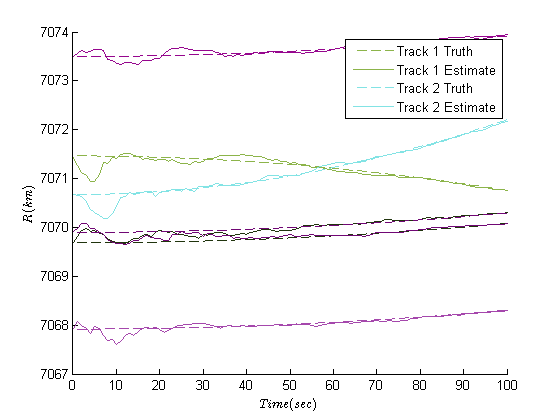
\includegraphics[width=0.45\columnwidth]{JPDAF_Radii_Tracks1234}}
	\subfigure[\;JPDAF Uncertainty]
		{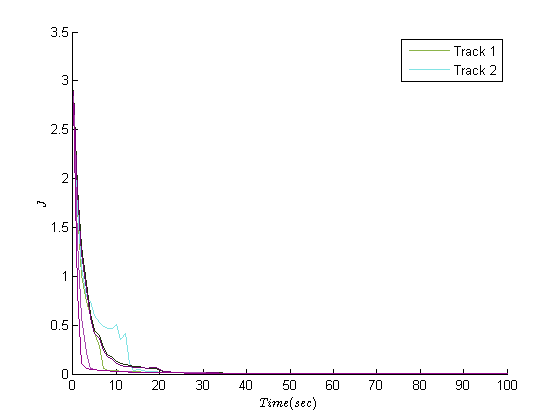
\includegraphics[width=0.45\columnwidth]{JPDAF_UncertaintyCosts_Tracks1234}}
	}
\centerline{
	\subfigure[\;O-JPDAF Radii]
		{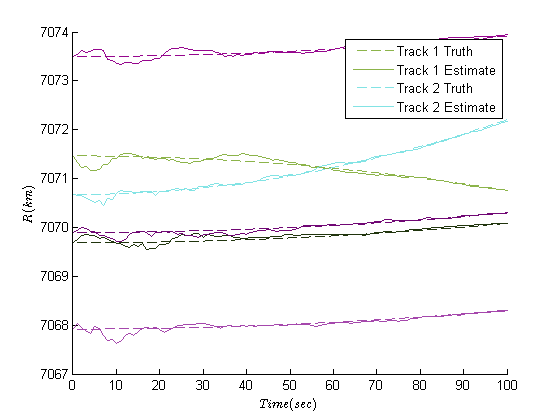
\includegraphics[width=0.45\columnwidth]{O-JPDAF_Radii_Tracks1234}}
	\subfigure[\;O-JPDAF Uncertainty]
		{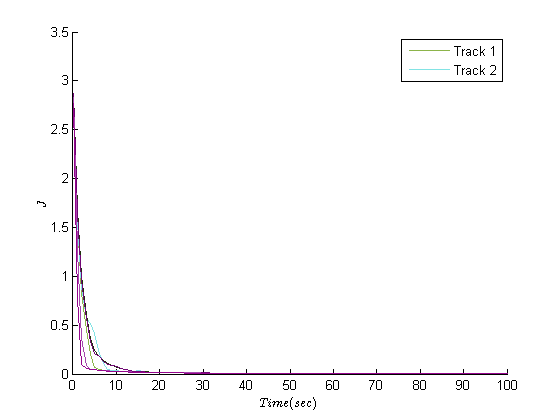
\includegraphics[width=0.45\columnwidth]{O-JPDAF_UncertaintyCosts_Tracks1234}}
	}
\centerline{
	\subfigure[\;Comparison of Radii of the First Two Tracks]
		{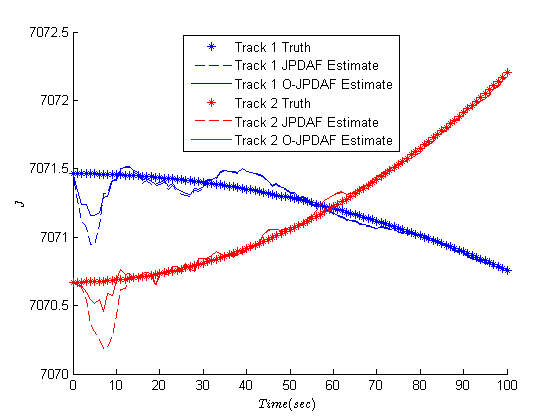
\includegraphics[width=0.45\columnwidth]{ComparisonRadii_Tracks12}}
	\subfigure[\;Comparison of Uncertainties of the First Two Tracks]
		{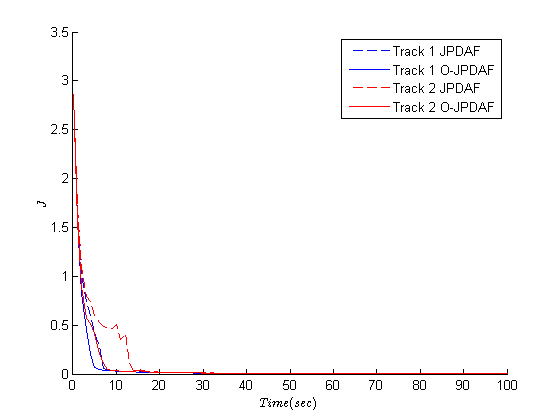
\includegraphics[width=0.45\columnwidth]{ComparisonUncertaintyCosts_Tracks12}}
	}
\caption{The orbital radii and costs are compared among the algorithms to show that their is a small improvement in the mean of the estimates with the O-JPDAF and large improvement in the uncertainty in the estimates. Addtitionally, both algorithms handled an uncertain number of measurements and false alarms in these simulations.
}\label{fig:hoverRegions}
\end{figure}











%\\
%P^+_{i}=&P^-_{i}+K_i\{(1-\beta_{0,i})S_i+({\sum\limits_{j} \beta_{ij}e_{ij}e_{ij}^T-{\bf{e_{ij}}}}{\bf{e_{ij}}}^T)\}K_{i}^T
%\\
%P^+_{i}=&P^-_{i}+K_iS^*K_i^T, \quad S^*=(1-\beta_{0,i})S_i+({\sum\limits_{j} \beta_{ij}e_{ij}e_{ij}^T-{\bf{e_{ij}}}}{\bf{e_{ij}}}^T)



















%
%
\section{Coalescence Avoiding Optimal Joint Probabilistic Data Association Filter (C-JPDAF)}% Or another name that you choose
\label{C-JPDAF}

The O-JPDAF described in the previous section is effective in handling clutter or missed detection of multiple objects. However, it is prone to coalescing estimates, especially with objects in close-proximity. Here, we present a coalescence-avoiding optimal JPDAF, hereafter C-JPDAF for short, to avoid coalescence of the estimates. The main idea is choosing the estimator gain such that a weighted sum of the size of uncertainty and a measure of similarity is minimized. 

A similarity measure is introduced first, and an optimization problem is formulated. Throughout this section, the subscript $k$ denoting the time step is omitted for simplicity. 


	
\subsection{Matusita's Similarity Measure}

Coalescence of neighboring estimates only occurs when these estimates are very similar. We evaluate the Matusita's measure of similarity because it takes the form of a differentiable analytic index. For two Gaussian probability density functions, $f_1(x)$ and $f_2(x)$, Matusita's measure is defined as
\begin{align*}
\zeta = \int \sqrt{f_1(x)f_2(x)}dx,
\end{align*}
which is between 0 and 1, and it measures the similarity between two densities ~\cite{Coal_k}. 

From~\cite{Coal_k}, using the assumption that the a posteriori states $\hat x_\mathcal{A}^+$ and $\hat x_\mathcal{B}^+$ are Gaussian, the Matusita's measure between two objects can be written as
\begin{align}
\zeta=\zeta_1\zeta_2,
\end{align}
where
\begin{align}
\label{Q}
\zeta_1=&\frac{2^\frac{n}{2}|P_\mathcal{A}^+|^{\frac{1}{4}}|P_\mathcal{B}^+|^{\frac{1}{4}}}{|P_\mathcal{A}^++P_\mathcal{B}^+|^{\frac{1}{2}}},
\end{align}
\begin{align}
\label{R}
\zeta_2=&\exp{\left\{-\frac{1}{4}(\hat x^+_\mathcal{A}-\hat x^+_\mathcal{B})^T(P_\mathcal{A}^++P_\mathcal{B}^+)^{-1}(\hat x^+_\mathcal{A}-\hat x^+_\mathcal{B})\right\}}.
\end{align}
Here $\zeta_1$ measures the differences in the covariances and $\zeta_2$ represents the spread in the means.

%Coalescence is well known to occur when estimates share measurements over long periods of time; estimates with largely different state covariances do not tend to coalesce
%; consider two satellites $1$ and $2$ such that $S_1>>S_2$. Inside the measurement space, if a measurement falls nearby $\hat z_1$, then estimate with low measurement uncertainty...
	% Introduce the definition of M-measure
	% Introduce the definition of Bhattacharyya distance
	
\subsection{Optimal Coalescence Avoidance}

Define a cost function of coalescence avoiding filtering as

\begin{align}
J=J_P+cJ_S
\end{align}
where $J_P$ is an uncertainty cost that measures the confidence level of estimation and $J_S$ is a similarity cost that measures degree of coalescence. The constant $c$ is a positive weighting factor between $J_P$ and $J_S$. 

In the proposed C-JPDAF, the a posteriori estimate of the state is given in the form of O-JPDA given by \refeqn{GainK}, but the estimator gain $K_i$ is selected to minimize the total cost $J$. In short, the estimator gain is chosen in the consideration of both uncertainty and coalescence. These are illustrated at Figure \ref{fig:CostTrends}.

\begin{figure}
\setlength{\unitlength}{0.1\columnwidth}
\centerline{\footnotesize\selectfont
\begin{picture}(8.5,7.3)(-0.5,-0.8)
\put(-0.5,3){\rotatebox{90}{Cost}}
\put(0,0){\includegraphics[width=0.8\columnwidth]{ECC14_fig1.pdf}}
\put(6.2,0.2){\shortstack[c]{Uncertainty\\ cost: $J_P$}}
\put(6.2,2.8){\shortstack[c]{Similarity\\ cost: $J_S$}}
\put(5.7,5.2){\shortstack[c]{Weighted sum:\\ $J=J_P+cJ_S$}}
\put(4.98,0.78){\circle*{0.1}}
\put(2.48,1.57){\circle*{0.1}}
\put(5.0,-0.3){$K_{O-JPDAF}$}
\put(2.5,-0.3){$K_{C-JPDAF}$}
\put(3.1,-0.8){Estimator gain}
\end{picture}
}
\caption{Illustration of optimal coalescence avoidance: several costs are illustrated with respect to an element of an estimator gain $K$ (red: uncertainty cost $J_P$, blue: similarity cost $J_S$, black: weighted sum). The estimator gain $K_{O-JPDAF}$ of O-JPDAF is selected to minimize the uncertainty cost. In the proposed approach, the estimator gain $K_{C-JPDAF}$ is chosen such that the weighted sum of the uncertainty cost and the similarity cost is minimized. In short, at the expense of increased uncertainty at a single step, the proposed approach prevents coalescence. The increased uncertainty at each step is rewarded by reducing the overall estimation error drastically by maintaining correct data association throughout crossing tracks in close proximity.}
\label{fig:CostTrends}
\end{figure}

More explicitly, the uncertainty cost $J_P$ is defined as the sum of the trace of each a posteriori covariance:
\begin{align}
J_P=\sum\limits_{i}^{t}\tr{P^+_i},\label{eqn:JP}
\end{align}
where $P^+_{i}$ is obtained by \refeqn{JPDAFCov}. The similarity cost is chosen as the second part of the Matusita's measure that represents the weighted-spread of the mean values:
\begin{align}
J_S&=\sum\limits_{\mathcal{A}}^{t}\sum\limits_{\mathcal{B}}^{t}\exp (-au_{\mathcal{A}\mathcal{B}})\bigg|_{\mathcal{A}\neq\mathcal{B}}\\
u_{\mathcal{A}\mathcal{B}} & = \begin{cases} (\hat x_{\mathcal{A}}^+-\hat x^+_{\mathcal{B}})^T(P^+_{\mathcal{A}}+P^+_{\mathcal{B}})^{-1}(\hat x^+_{\mathcal{A}}-\hat x^+_{\mathcal{B}})\label{eqn:u}, & \mbox{if } \zeta_2^->\zeta_{2,min} \\ 0 & \mbox{otherwise}  \end{cases}
\end{align}
%%%% \norm{\hat x_{\mathcal{A}}^+-\hat x^+_{\mathcal{B}}}
% OR
%\begin{align}
%J_S&=\sum\limits_{\mathcal{A}}^{t}\sum\limits_{\mathcal{B}}^{t}\exp (-au_{\mathcal{A}\mathcal{B}})\bigg|_{\mathcal{A}\neq\mathcal{B}}\\
%u_{\mathcal{A}\mathcal{B}} & = (\hat x_{\mathcal{A}}^+-\hat x^+_{\mathcal{B}})^T(P^+_{\mathcal{A}}+P^+_{\mathcal{B}})^{-1}(\hat x^+_{\mathcal{A}}-\hat x^+_{\mathcal{B}})
%\end{align}
where $\zeta_2^-$ is calculated using $\hat x^-_{\mathcal A}$ and $\hat x^-_{\mathcal B}$ as the means and $P^-_\mathcal{A}$ and $P^-_\mathcal{B}$ as the covariances, $\zeta_{2,min}$ defines a region of separation, and positive constant $a$ serves to amplify or attenuate the function as well as alter its shape.

Necessary conditions for optimality are given by
\begin{align}
\deriv{J}{K_i} = \deriv{J_P}{K_i} + c \deriv{J_S}{K_i} =0,\label{eqn:NCO}
\end{align}
where $\deriv{J_S}{K_i}$ may be nonzero. These are solved for the set of all gains $\mathcal{K}=\{K_1,K_2,...,K_t\}$. 


Next, we find the derivative of each cost. The derivative of $J_P$ is taken from \refeqn{Uncertainty0}
\begin{align}
\label{eqn:CostP}
\frac{\partial J_{P}}{\partial K_{i}}&=2K_iE_i-2(1-\beta_{0,i})P^-_iH_i^T
\end{align}
Note that $J_{P_\mathcal{X}}$ does not depend on $K_\mathcal{Y}$ for $\mathcal{X}\neq \mathcal{Y}$.

%
%To appropriately define the similarity cost, we only consider the $R$ term from Equation \ref{R} because coalescence is well known to occur when estimates are within close proximity. For simplicity, we define ${P^+_{12}}^{-1}$ as
%\begin{align}
%{P^+_{12}}^{-1}=(P_1^++P_2^+)^{-1}
%\end{align}
%and define define $u$ as
We expand the nonzero portion of \refeqn{u} so it may be differentiated with respect to $K_\mathcal{A}$,
\begin{align}
\begin{split}
u=&(\hat x^+_\mathcal{A}-\hat x^+_\mathcal{B})^T{P^+_{\mathcal{A}\mathcal{B}}}^{-1}(\hat x^+_\mathcal{A}-\hat x^+_\mathcal{B})
\\
=&\hat x^{+T}_\mathcal{A}{P^+_{\mathcal{A}\mathcal{B}}}^{-1}\hat x^+_\mathcal{A}
-2\hat x^{+T}_\mathcal{B}{P^+_{\mathcal{A}\mathcal{B}}}^{-1}\hat x^+_\mathcal{A}
+\hat x^{+T}_\mathcal{B}{P^+_{\mathcal{A}\mathcal{B}}}^{-1}\hat x^+_\mathcal{B}
\\
=&(\hat x^-_\mathcal{A}+K_\mathcal{A}{\bf e}_\mathcal{A})^T{P^+_{\mathcal{A}\mathcal{B}}}^{-1}(\hat x^-_\mathcal{A}+K_\mathcal{A}{\bf e}_\mathcal{A})%
-2(\hat x^-_\mathcal{B}+K_\mathcal{B}{\bf e}_\mathcal{B})^T{P^+_{\mathcal{A}\mathcal{B}}}^{-1}(\hat x^-_\mathcal{A}+K_\mathcal{A}{\bf e}_\mathcal{A})
\\
&+(\hat x^-_\mathcal{B}+K_\mathcal{B}{\bf e}_\mathcal{B})^T{P^+_{\mathcal{A}\mathcal{B}}}^{-1}(\hat x^-_\mathcal{B}+K_\mathcal{B}{\bf e}_\mathcal{B})
\\
=&\hat x^{-T}_\mathcal{A}{P^+_{\mathcal{A}\mathcal{B}}}^{-1}\hat x^-_\mathcal{A}
+2\hat x^{-T}_\mathcal{A}{P^+_{\mathcal{A}\mathcal{B}}}^{-1}K_\mathcal{A}{\bf e}_\mathcal{A}
+{\bf e}_\mathcal{A}^TK_\mathcal{A}^T{P^+_{\mathcal{A}\mathcal{B}}}^{-1}K_\mathcal{A}{\bf e}_\mathcal{A}
\\
&+\hat x^{-T}_\mathcal{B}{P^+_{\mathcal{A}\mathcal{B}}}^{-1}\hat x^-_\mathcal{B}
+2\hat x^{-T}_\mathcal{B}{P^+_{\mathcal{A}\mathcal{B}}}^{-1}K_\mathcal{B}{\bf e}_\mathcal{B}
+{\bf e}_\mathcal{B}^TK_\mathcal{B}^T{P^+_{\mathcal{A}\mathcal{B}}}^{-1}K_\mathcal{B}{\bf e}_\mathcal{B}
\\
&-2\{\hat x^{-T}_\mathcal{B}{P^+_{\mathcal{A}\mathcal{B}}}^{-1}\hat x^-_\mathcal{A}
+\hat x^{-T}_\mathcal{B}{P^+_{\mathcal{A}\mathcal{B}}}^{-1}K_\mathcal{A}{\bf e}_\mathcal{A}
+\hat x^{-T}_\mathcal{A}{P^+_{\mathcal{A}\mathcal{B}}}^{-1}K_\mathcal{B}{\bf e}_\mathcal{B}
+{\bf e}_\mathcal{B}^TK_\mathcal{B}^T{P^+_{\mathcal{A}\mathcal{B}}}^{-1}K_\mathcal{A}{\bf e}_\mathcal{A}\}
\\
=&\hat x_\mathcal{A}^{-T}{P^+_{\mathcal{A}\mathcal{B}}}^{-1}\hat x_\mathcal{A}^-
-2\hat x_\mathcal{A}^{-T}{P^+_{\mathcal{A}\mathcal{B}}}^{-1}\hat x_\mathcal{B}^-
\\
&+2(\hat x_\mathcal{A}^{-}-\hat x_\mathcal{B}^{-})^T{P^+_{\mathcal{A}\mathcal{B}}}^{-1}K_\mathcal{A}{\bf e}_\mathcal{A}
+\hat x_\mathcal{B}^{-T}{P^+_{\mathcal{A}\mathcal{B}}}^{-1}\hat x_\mathcal{B}^-
\\
&+2(\hat x_\mathcal{B}^{-}-\hat x_\mathcal{A}^{-})^T{P^+_{\mathcal{A}\mathcal{B}}}^{-1}K_\mathcal{B}{\bf e}_\mathcal{B}
+{\bf e}_\mathcal{A}^TK_\mathcal{A}^T{P^+_{\mathcal{A}\mathcal{B}}}^{-1}K_\mathcal{A}{\bf e}_\mathcal{A}
\\
&-2{\bf e}_\mathcal{B}^TK_\mathcal{B}^T{P^+_{\mathcal{A}\mathcal{B}}}^{-1}K_\mathcal{A}{\bf e}_\mathcal{A}
+{\bf e}_\mathcal{B}^TK_\mathcal{B}^T{P^+_{\mathcal{A}\mathcal{B}}}^{-1}K_\mathcal{B}{\bf e}_\mathcal{B},
\label{eqn:uexpanded}
\end{split}
\end{align}
where ${P^+_{\mathcal{A}\mathcal{B}}}^{-1}=(P_\mathcal{A}^++P_\mathcal{B}^+)^{-1}$. 

%which is the most reduced form to differentiate with respect to $K_1$ and $K_2$.

\newcommand{\Iij}{\ensuremath{\mathbf{1}_{ij}}}

Let $\Iij\in \Re^{n\times m}$ be defined such that its $i,j$-th element is one and other elements are zero. The derivative of $(P_{\mathcal{A}\mathcal{B}}^+)^{-1}$ with respect to the $i,j$-th element of $K_\mathcal{A}$ is defined as $\mathcal{P}_{\mathcal{A}\mathcal{B}_{ij}}\in\Re^{n\times n}$:
%such that $ij1(i,j)=1$ and $0$ elsewhere, we define $P^*_{12}$ as
\begin{align}
\begin{split}
\mathcal{P}_{\mathcal{A}\mathcal{B}_{\mathcal{A},ij}}&=\frac{\partial {P^+_{\mathcal{A}\mathcal{B}}}^{-1}}{\partial K_{\mathcal{A},ij}}
\\
&=-{P_{\mathcal{A}\mathcal{B}}^+}^{-1}\frac{\partial}{\partial K_{\mathcal{A},ij}}
\left(
P^-_\mathcal{A}-(1-\beta_{0,\mathcal{A}})(K_\mathcal{A}H_\mathcal{A}P^-_\mathcal{A}+P^-_\mathcal{A}H_\mathcal{A}^TK_\mathcal{A}^T)+K_\mathcal{A}E_\mathcal{A}K_\mathcal{A}^T
\right)
{P_{\mathcal{A}\mathcal{B}}^+}^{-1}
\\
&={P_{\mathcal{A}\mathcal{B}}^+}^{-1}[(1-\beta_{0,\mathcal{A}})(\Iij H_\mathcal{A}P_\mathcal{A}^-+P_\mathcal{A}^-H_\mathcal{A}^T\Iij^T)-\Iij E_\mathcal{A}K_\mathcal{A}^T -K_\mathcal{A}E_\mathcal{A}\Iij^T]{P_{\mathcal{A}\mathcal{B}}^+}^{-1}.
\end{split}
\end{align}
Using this, the derivative of $u_{\mathcal{A}\mathcal{B}}$ with respect to the $i,j$-th element of $K_\mathcal{A}$ can be written as
\begin{align}
\begin{split}
\frac{\partial u_{\mathcal{A}\mathcal{B}}}{\partial K_{\mathcal{A},ij}}
=&\frac{\partial}{\partial K_{\mathcal{A},ij}}\{\hat x_\mathcal{A}^{-T}{P^+_{\mathcal{A}\mathcal{B}}}^{-1}\hat x_\mathcal{A}^-
-2\hat x_\mathcal{A}^{-T}{P^+_{\mathcal{A}\mathcal{B}}}^{-1}\hat x_\mathcal{B}^-
\\
&+2(\hat x_\mathcal{A}^{-}-\hat x_\mathcal{B}^{-})^T{P^+_{\mathcal{A}\mathcal{B}}}^{-1}K_\mathcal{A}{\bf e}_\mathcal{A}
+\hat x_\mathcal{B}^{-T}{P^+_{\mathcal{A}\mathcal{B}}}^{-1}\hat x_\mathcal{B}^-
\\
&+2(\hat x_\mathcal{B}^{-}-\hat x_\mathcal{A}^{-})^T{P^+_{\mathcal{A}\mathcal{B}}}^{-1}K_\mathcal{B}{\bf e}_\mathcal{B}
+{\bf e}_\mathcal{A}^TK_\mathcal{A}^T{P^+_{\mathcal{A}\mathcal{B}}}^{-1}K_\mathcal{A}{\bf e}_\mathcal{A}
\\
&-2{\bf e}_\mathcal{B}^TK_\mathcal{B}^T{P^+_{\mathcal{A}\mathcal{B}}}^{-1}K_\mathcal{A}{\bf e}_\mathcal{A}
+{\bf e}_\mathcal{B}^TK_\mathcal{B}^T{P^+_{\mathcal{A}\mathcal{B}}}^{-1}K_\mathcal{B}{\bf e}_\mathcal{B}\}
\\
=& \hat x_\mathcal{A}^{-T}\mathcal{P}_{\mathcal{A}\mathcal{B}_{\mathcal{A},ij}}\hat x_\mathcal{A}^-
-2\hat x_\mathcal{A}^{-T}\mathcal{P}_{\mathcal{A}\mathcal{B}_{\mathcal{A},ij}}\hat x_\mathcal{B}^-
\\
&+2(\hat x_\mathcal{A}^{-}-\hat x_\mathcal{B}^{-})^T
[\mathcal{P}_{\mathcal{A}\mathcal{B}_{\mathcal{A},ij}}K_\mathcal{A}+{P^+_{\mathcal{A}\mathcal{B}}}^{-1}\Iij]
{\bf e}_\mathcal{A}
\\
&+\hat x_\mathcal{B}^{-T}\mathcal{P}_{\mathcal{A}\mathcal{B}_{\mathcal{A},ij}}\hat x_\mathcal{B}^-
+2(\hat x_\mathcal{B}^{-}-\hat x_\mathcal{A}^{-})^T\mathcal{P}_{\mathcal{A}\mathcal{B}_{\mathcal{A},ij}}K_\mathcal{B}{\bf e}_\mathcal{B}
\\
&+{\bf e}_\mathcal{A}^T[\Iij^T{P^+_{\mathcal{A}\mathcal{B}}}^{-1}K_\mathcal{A}
+K_\mathcal{A}^T\mathcal{P}_{\mathcal{A}\mathcal{B}_{\mathcal{A},ij}}K_\mathcal{A}
\\
&+K_\mathcal{A}^T{P^+_{\mathcal{A}\mathcal{B}}}^{-1}\Iij]{\bf e}_\mathcal{A}
-2{\bf e}_\mathcal{B}^TK_\mathcal{B}^T[\mathcal{P}_{\mathcal{A}\mathcal{B}_{\mathcal{A},ij}}K_\mathcal{A}
\\
&+{P^+_{\mathcal{A}\mathcal{B}}}^{-1}\Iij]{\bf e}_\mathcal{A}
+{\bf e}_\mathcal{B}^TK_\mathcal{B}^T\mathcal{P}_{\mathcal{A}\mathcal{B}_{\mathcal{A},ij}}K_\mathcal{B}{\bf e}_\mathcal{B}.
\end{split}
\end{align}
From this, the derivation of the similarity cost $J_S$ with respect to the $i,j$-th element of $K_\mathcal{A}$ is given by
\begin{align}
\frac{\partial J_{S}}{\partial K_{\mathcal{A},ij}}=-a\exp(-au_{\mathcal{A}\mathcal{B}})\frac{\partial u_{\mathcal{A}\mathcal{B}}}{\partial K_{\mathcal{A},ij}}.\label{eqn:JSK}
\end{align}

In summary, \refeqn{CostP} and \refeqn{JSK} are substituted into \refeqn{NCO}, and it is solved to obtain the set of optimal gains $\mathcal{K}$. Then, the algorithm of C-JPDAF is completed by updating the state estimate and covariance by using \refeqn{KalEst} and \refeqn{JPDAFCov}, respectively.


As the optimality condition is a nonlinear function of estimator gains, there is no closed-form solution. Hence, we require a nonlinear equation solver. Note that ${P_\mathcal{A}^+}^{-1}$, ${P_\mathcal{B}^+}^{-1}$, and ${P_{\mathcal{A}\mathcal{B}}^+}^{-1}$ are symmetric inverses and must only be calculated once for each $(\mathcal{A},\mathcal{B})$ where the similarity measure is nontrivial. When $c=0$, we can show that the optimal gain reduces to that of the O-JPDAF, which is used as an initial guess of numerical solutions.

%\subsection{Suboptimal Solution}
%Because optimal solution of \ref{eqn:JSK} does not have a closed-form solution, a close initial guess to the actual solution can decrease the computational requirements of the problem. Therefore for objects $1$ and $2$, we can minimize the two equations:
%\begin{align}
%\frac{\partial J}{\partial K_1}
%&=\frac{\partial J_{P}}{\partial K_1}+c\frac{\partial J_{S}}{\partial K_1}
%\approx2\beta_1({K_1S_1-P_1^-H_1^T})-ac\exp(-au^-)\frac{\partial u^*}{\partial K_1}
%\label{eqn:subopt1}\\
%\frac{\partial J}{\partial K_2}
%&=\frac{\partial J_{P}}{\partial K_2}+c\frac{\partial J_{S}}{\partial K_2}
%\approx2\beta_2({K_2S_2-P_2^-H_2^T})-ac\exp(-au^-)\frac{\partial u^*}{\partial K_2}
%\label{eqn:subopt2}
%\end{align}
%where
%\begin{align}
%u^-&= (\hat x^-_1-\hat x^-_2)^T(P^-_{1}+P^-_{2})^{-1}(\hat x^-_1-\hat x^-_2)\label{eqn:uminus}\\
%u^*&= (\hat x^+_1-\hat x^+_2)^T(P^-_{1}+P^-_{2})^{-1}(\hat x^+_1-\hat x^+_2)\label{eqn:uminus}
%\end{align}
%so that we define a new variable $\Omega=ac\exp(-au^-)$, which may be treated as constant in \ref{eqn:subopt1} and \ref{eqn:subopt2}. We modify \ref{eqn:uexpanded} to solve for $u^*$,
%\begin{align}
%\label{eqn:ustarexpanded}
%u^*=&\{\hat x_1^{-T}{P^-_{12}}^{-1}\hat x_1^-
%-2\hat x_1^{-T}{P^-_{12}}^{-1}\hat x_2^-\nonumber\\
%&+2\beta_1(\hat x_1^{-}-\hat x_2^{-})^T{P^-_{12}}^{-1}K_1e_1
%+\hat x_2^{-T}{P^-_{12}}^{-1}\hat x_2^-\nonumber\\
%&+2\beta_2(\hat x_2^{-}-\hat x_1^{-})^T{P^-_{12}}^{-1}K_2e_2
%+\beta_1^2e_1^TK_1^T{P^-_{12}}^{-1}K_1e_1\nonumber\\
%&-2\beta_1\beta_2e_2^TK_2^T{P^-_{12}}^{-1}K_1e_1
%+\beta_2^2e_2^TK_2^T{P^-_{12}}^{-1}K_2e_2\}
%\end{align}
%where ${P^-_{12}}^{-1}=(P_1^-+P_2^-)^{-1}$, which is fixed with respect to $K_1$ and $K_2$. We take the derivative of \ref{eqn:ustarexpanded} with respect to $K_1$ and $K_2$
%\begin{align}
%\begin{split}
%\frac{\partial u^*}{\partial K_1}=&\frac{\partial}{\partial K_1}\left(2\beta_1(\hat x_1^{-}-\hat x_2^{-})^T{P^-_{12}}^{-1}K_1e_1
%+\beta_1^2e_1^TK_1^T{P^-_{12}}^{-1}K_1e_1
%-2\beta_1\beta_2e_2^TK_2^T{P^-_{12}}^{-1}K_1e_1\right)\\
%=&2\beta_1{P^-_{12}}^{-1}(\hat x_1^{-}-\hat x_2^{-})e_1^T
%+2\beta_1^2{P^-_{12}}^{-1}K_1e_1e_1^T
%-2\beta_1\beta_2{P^-_{12}}^{-1}K_2e_2e_1^T.
%\label{eqn:ustarderivexpanded}
%\end{split}
%\end{align}
%Let $\lambda$ be an eigenvalue of ${P^-_{12}}^{-1}$ and $q$ be the associated eigenvector, i.e. ${P^-_{12}}^{-1}q=\lambda q\Rightarrow q^T{P^-_{12}}^{-1}=\lambda q^T$ because ${P^-_{12}}^{-1}$ is symmetric.
%Then the derviative of \ref{eqn:ustarexpanded} with resepect to $K_1$ and $K_2$ and setting this to zero yields
%\begin{align}
%0&=2\beta_1({K_1S_1-P_1^-H_1^T})-\Omega\frac{\partial u^*}{\partial K_1}\\
%0&=2\beta_1({K_1S_1-P_1^-H_1^T})-2\beta_1\Omega\left(
%{P^-_{12}}^{-1}(\hat x_1^{-}-\hat x_2^{-})e_1^T
%+\beta_1{P^-_{12}}^{-1}K_1e_1e_1^T
%-\beta_2{P^-_{12}}^{-1}K_2e_2e_1^T\right)\\
%0&=K_1S_1-P_1^-H_1^T
%-\Omega{P^-_{12}}^{-1}(\hat x_1^{-}-\hat x_2^{-})e_1^T
%-\Omega\beta_1{P^-_{12}}^{-1}K_1e_1e_1^T
%+\Omega\beta_2{P^-_{12}}^{-1}K_2e_2e_1^T\\
%0&=q^TK_1S_1-q^TP_1^-H_1^T
%-\Omega q^T{P^-_{12}}^{-1}(\hat x_1^{-}-\hat x_2^{-})e_1^T
%-\Omega\beta_1q^T{P^-_{12}}^{-1}K_1e_1e_1^T
%+\Omega\beta_2q^T{P^-_{12}}^{-1}K_2e_2e_1^T\\
%0&=q^TK_1S_1-q^TP_1^-H_1^T
%-\Omega q^T\lambda(\hat x_1^{-}-\hat x_2^{-})e_1^T
%-\Omega\beta_1q^T\lambda K_1e_1e_1^T
%+\Omega\beta_2q^T\lambda K_2e_2e_1^T\\
%0&=q^T\left\{K_1S_1-P_1^-H_1^T
%-\Omega\lambda(\hat x_1^{-}-\hat x_2^{-})e_1^T
%-\Omega\beta_1\lambda K_1e_1e_1^T
%+\Omega\beta_2\lambda K_2e_2e_1^T\right\},
%\quad q\neq0\\
%0&=K_1(S_1-\Omega\beta_1\lambda e_1e_1^T)
%-P_1^-H_1^T
%-\Omega\lambda(\hat x_1^{-}-\hat x_2^{-})e_1^T
%+\Omega\beta_2\lambda K_2e_2e_1^T\\
%K_1&=\left(P_1^-H_1^T
%+\Omega\lambda(\hat x_1^{-}-\hat x_2^{-})e_1^T
%-\Omega\beta_2\lambda K_2e_2e_1^T\right)
%(S_1-\Omega\beta_1\lambda e_1e_1^T)^{-1}
%\label{eqn:K1coupled}
%\end{align}
%and similarly
%\begin{align}
%K_2&=\left(P_2^-H_2^T
%+\Omega\lambda(\hat x_2^{-}-\hat x_1^{-})e_2^T
%-\Omega\beta_1\lambda K_1e_1e_2^T\right)
%(S_2-\Omega\beta_2\lambda e_2e_2^T)^{-1}
%\label{eqn:K2coupled}.
%\end{align}
%The equations \ref{eqn:K1coupled} and \ref{eqn:K2coupled} may be substituted into each other to seclude $K_1$ and $K_2$
%\begin{align}
%\begin{split}
%K_1&=(P_1^-H_1^T
%+\Omega\lambda(\hat x_1^{-}-\hat x_2^{-})e_1^T
%-\Omega\beta_2\lambda[P_2^-H_2^T
%+\Omega\lambda(\hat x_2^{-}-\hat x_1^{-})e_2^T\\
%&-\Omega\beta_1\lambda K_1e_1e_2^T]
%(S_2-\Omega\beta_2\lambda e_2e_2^T)^{-1}e_2e_1^T)
%(S_1-\Omega\beta_1\lambda e_1e_1^T)^{-1}
%\end{split}
%\end{align}
%which may be rearranged to
%\begin{align}
%\begin{split}
%&K_1\left(I-\Omega^2\lambda^2\beta_1\beta_2e_1e_2^T(S_2-\Omega\beta_2\lambda e_2e_2^T)^{-1}e_2e_1^T
%(S_1-\Omega\beta_1\lambda e_1e_1^T)^{-1}\right)=(P_1^-H_1^T
%+\Omega\lambda(\hat x_1^{-}-\hat x_2^{-})e_1^T\\
%&-\Omega\beta_2\lambda[P_2^-H_2^T+\Omega\lambda(\hat x_2^{-}-\hat x_1^{-})e_2^T](S_2-\Omega\beta_2\lambda e_2e_2^T)^{-1}e_2e_1^T)
%(S_1-\Omega\beta_1\lambda e_1e_1^T)^{-1}.
%\end{split}
%\end{align}
%Solving for $K_1$,
%\begin{align}
%\begin{split}
%K_1=&(P_1^-H_1^T
%+\Omega\lambda(\hat x_1^{-}-\hat x_2^{-})e_1^T
%-\Omega\beta_2\lambda[P_2^-H_2^T+\Omega\lambda(\hat x_2^{-}-\hat x_1^{-})e_2^T]
%(S_2-\Omega\beta_2\lambda e_2e_2^T)^{-1}
%e_2e_1^T)
%(S_1-\\
%&\Omega\beta_1\lambda e_1e_1^T)^{-1}\left(I-\Omega^2\lambda^2\beta_1\beta_2e_1e_2^T(S_2-\Omega\beta_2\lambda e_2e_2^T)^{-1}e_2e_1^T
%(S_1-\Omega\beta_1\lambda e_1e_1^T)^{-1}\right)^{-1}
%\end{split}
%\end{align}
%and similarly
%\begin{align}
%\begin{split}
%K_2=&(P_2^-H_2^T
%+\Omega\lambda(\hat x_2^{-}-\hat x_1^{-})e_2^T
%-\Omega\beta_1\lambda[P_1^-H_1^T+\Omega\lambda(\hat x_1^{-}-\hat x_2^{-})e_1^T]
%(S_1-\Omega\beta_1\lambda e_1e_1^T)^{-1}
%e_1e_2^T)
%(S_2-\\
%&\Omega\beta_2\lambda e_2e_2^T)^{-1}\left(I-\Omega^2\lambda^2\beta_2\beta_1e_2e_1^T(S_1-\Omega\beta_1\lambda e_1e_1^T)^{-1}e_1e_2^T
%(S_2-\Omega\beta_2\lambda e_2e_2^T)^{-1}\right)^{-1}.
%\end{split}
%\end{align}


\bibliography{BibMaster}
\bibliographystyle{IEEEtran}

\end{document}















%\begin{align}
%\begin{split}
%u=&(\hat x^+_\mathcal{A}-\hat x^+_\mathcal{B})^T{P^+_{\mathcal{A}\mathcal{B}}}^{-1}(\hat x^+_\mathcal{A}-\hat x^+_\mathcal{B})
%\end{split}
%\\
%\begin{split}
%=&\hat x^{+T}_\mathcal{A}{P^+_{\mathcal{A}\mathcal{B}}}^{-1}\hat x^+_\mathcal{A}
%-2\hat x^{+T}_\mathcal{B}{P^+_{\mathcal{A}\mathcal{B}}}^{-1}\hat x^+_\mathcal{A}
%+\hat x^{+T}_\mathcal{B}{P^+_{\mathcal{A}\mathcal{B}}}^{-1}\hat x^+_\mathcal{B}
%\end{split}
%\\
%\begin{split}
%=&(\hat x^-_\mathcal{A}+K_\mathcal{A}{\bf e}_\mathcal{A})^T{P^+_{\mathcal{A}\mathcal{B}}}^{-1}(\hat x^-_\mathcal{A}+K_\mathcal{A}{\bf e}_\mathcal{A})%
%-2(\hat x^-_\mathcal{B}+\beta_\mathcal{B}K_\mathcal{B}e_\mathcal{B})^T{P^+_{\mathcal{A}\mathcal{B}}}^{-1}(\hat x^-_\mathcal{A}+K_\mathcal{A}{\bf e}_\mathcal{A})
%\\
%&+(\hat x^-_\mathcal{B}+\beta_\mathcal{B}K_\mathcal{B}e_\mathcal{B})^T{P^+_{\mathcal{A}\mathcal{B}}}^{-1}(\hat x^-_\mathcal{B}+\beta_\mathcal{B}K_\mathcal{B}e_\mathcal{B})
%\end{split}
%\\
%\begin{split}
%=&\hat x^{-T}_\mathcal{A}{P^+_{\mathcal{A}\mathcal{B}}}^{-1}\hat x^-_\mathcal{A}+2\hat x^{-T}_\mathcal{A}{P^+_{\mathcal{A}\mathcal{B}}}^{-1}\beta_\mathcal{A}K_\mathcal{A}e_\mathcal{A}
%+e_\mathcal{A}^TK_\mathcal{A}^T\beta_\mathcal{A}^T{P^+_{\mathcal{A}\mathcal{B}}}^{-1}K_\mathcal{A}{\bf e}_\mathcal{A}
%\\
%&+\hat x^{-T}_\mathcal{B}{P^+_{\mathcal{A}\mathcal{B}}}^{-1}\hat x^-_\mathcal{B}+2\hat x^{-T}_\mathcal{B}{P^+_{\mathcal{A}\mathcal{B}}}^{-1}\beta_\mathcal{B}K_\mathcal{B}e_\mathcal{B}+e_\mathcal{B}^TK_\mathcal{B}^T\beta_\mathcal{B}^T{P^+_{\mathcal{A}\mathcal{B}}}^{-1}\beta_\mathcal{B}K_\mathcal{B}e_\mathcal{B}
%\\
%&-2\{\hat x^{-T}_\mathcal{B}{P^+_{\mathcal{A}\mathcal{B}}}^{-1}\hat x^-_\mathcal{A}+\hat x^{-T}_\mathcal{B}{P^+_{\mathcal{A}\mathcal{B}}}^{-1}\beta_\mathcal{A}K_\mathcal{A}e_\mathcal{A}+\hat x^{-T}_\mathcal{A}{P^+_{\mathcal{A}\mathcal{B}}}^{-1}\beta_\mathcal{B}K_\mathcal{B}e_\mathcal{B}+e_\mathcal{B}^TK_\mathcal{B}^T\beta_\mathcal{B}^T{P^+_{\mathcal{A}\mathcal{B}}}^{-1}\beta_\mathcal{A}K_\mathcal{A}e_\mathcal{A}\}
%\end{split}
%\\
%\begin{split}
%=&\{\hat x_\mathcal{A}^{-T}{P^+_{\mathcal{A}\mathcal{B}}}^{-1}\hat x_\mathcal{A}^-
%-2\hat x_\mathcal{A}^{-T}{P^+_{\mathcal{A}\mathcal{B}}}^{-1}\hat x_\mathcal{B}^-
%\\
%&+2\beta_\mathcal{B}(\hat x_\mathcal{A}^{-}-\hat x_\mathcal{B}^{-})^T{P^+_{\mathcal{A}\mathcal{B}}}^{-1}K_\mathcal{A}e_\mathcal{A}
%+\hat x_\mathcal{B}^{-T}{P^+_{\mathcal{A}\mathcal{B}}}^{-1}\hat x_\mathcal{B}^-
%\\
%&+2\beta_\mathcal{B}(\hat x_\mathcal{B}^{-}-\hat x_\mathcal{A}^{-})^T{P^+_{\mathcal{A}\mathcal{B}}}^{-1}K_\mathcal{B}e_\mathcal{B}
%+\beta_\mathcal{A}^2e_\mathcal{A}^TK_\mathcal{A}^T{P^+_{\mathcal{A}\mathcal{B}}}^{-1}K_\mathcal{A}e_\mathcal{A}
%\\
%&-2\beta_\mathcal{A}\beta_\mathcal{B}e_\mathcal{B}^TK_\mathcal{B}^T{P^+_{\mathcal{A}\mathcal{B}}}^{-1}K_\mathcal{A}e_\mathcal{A}
%+\beta_\mathcal{B}^2e_\mathcal{B}^TK_\mathcal{B}^T{P^+_{\mathcal{A}\mathcal{B}}}^{-1}K_\mathcal{B}e_\mathcal{B}\},
%\label{eqn:uexpanded}
%\end{split}
%\end{align}














